\documentclass[12pt]{article}
\usepackage{graphicx}
\usepackage{float}
\begin{document}
\title{Electrical Engineering 141, Homework 5}
\date{February 22nd, 2019}
\author{Michael Wu\\UID: 404751542}
\maketitle

\section*{Problem 1}

\paragraph{a)}

This can be rewritten as follows.
\[L(s)=\frac{1}{200}\times\frac{1}{s}\times\frac{1}{s+1}\times\frac{1}{\frac{1}{100}s+1}\times\left(\frac{1}{5}s+1\right)\times\left(\frac{1}{10}s+1\right)\]
My asymptote sketch is shown below.
\begin{figure}[H]
    \begin{center}
        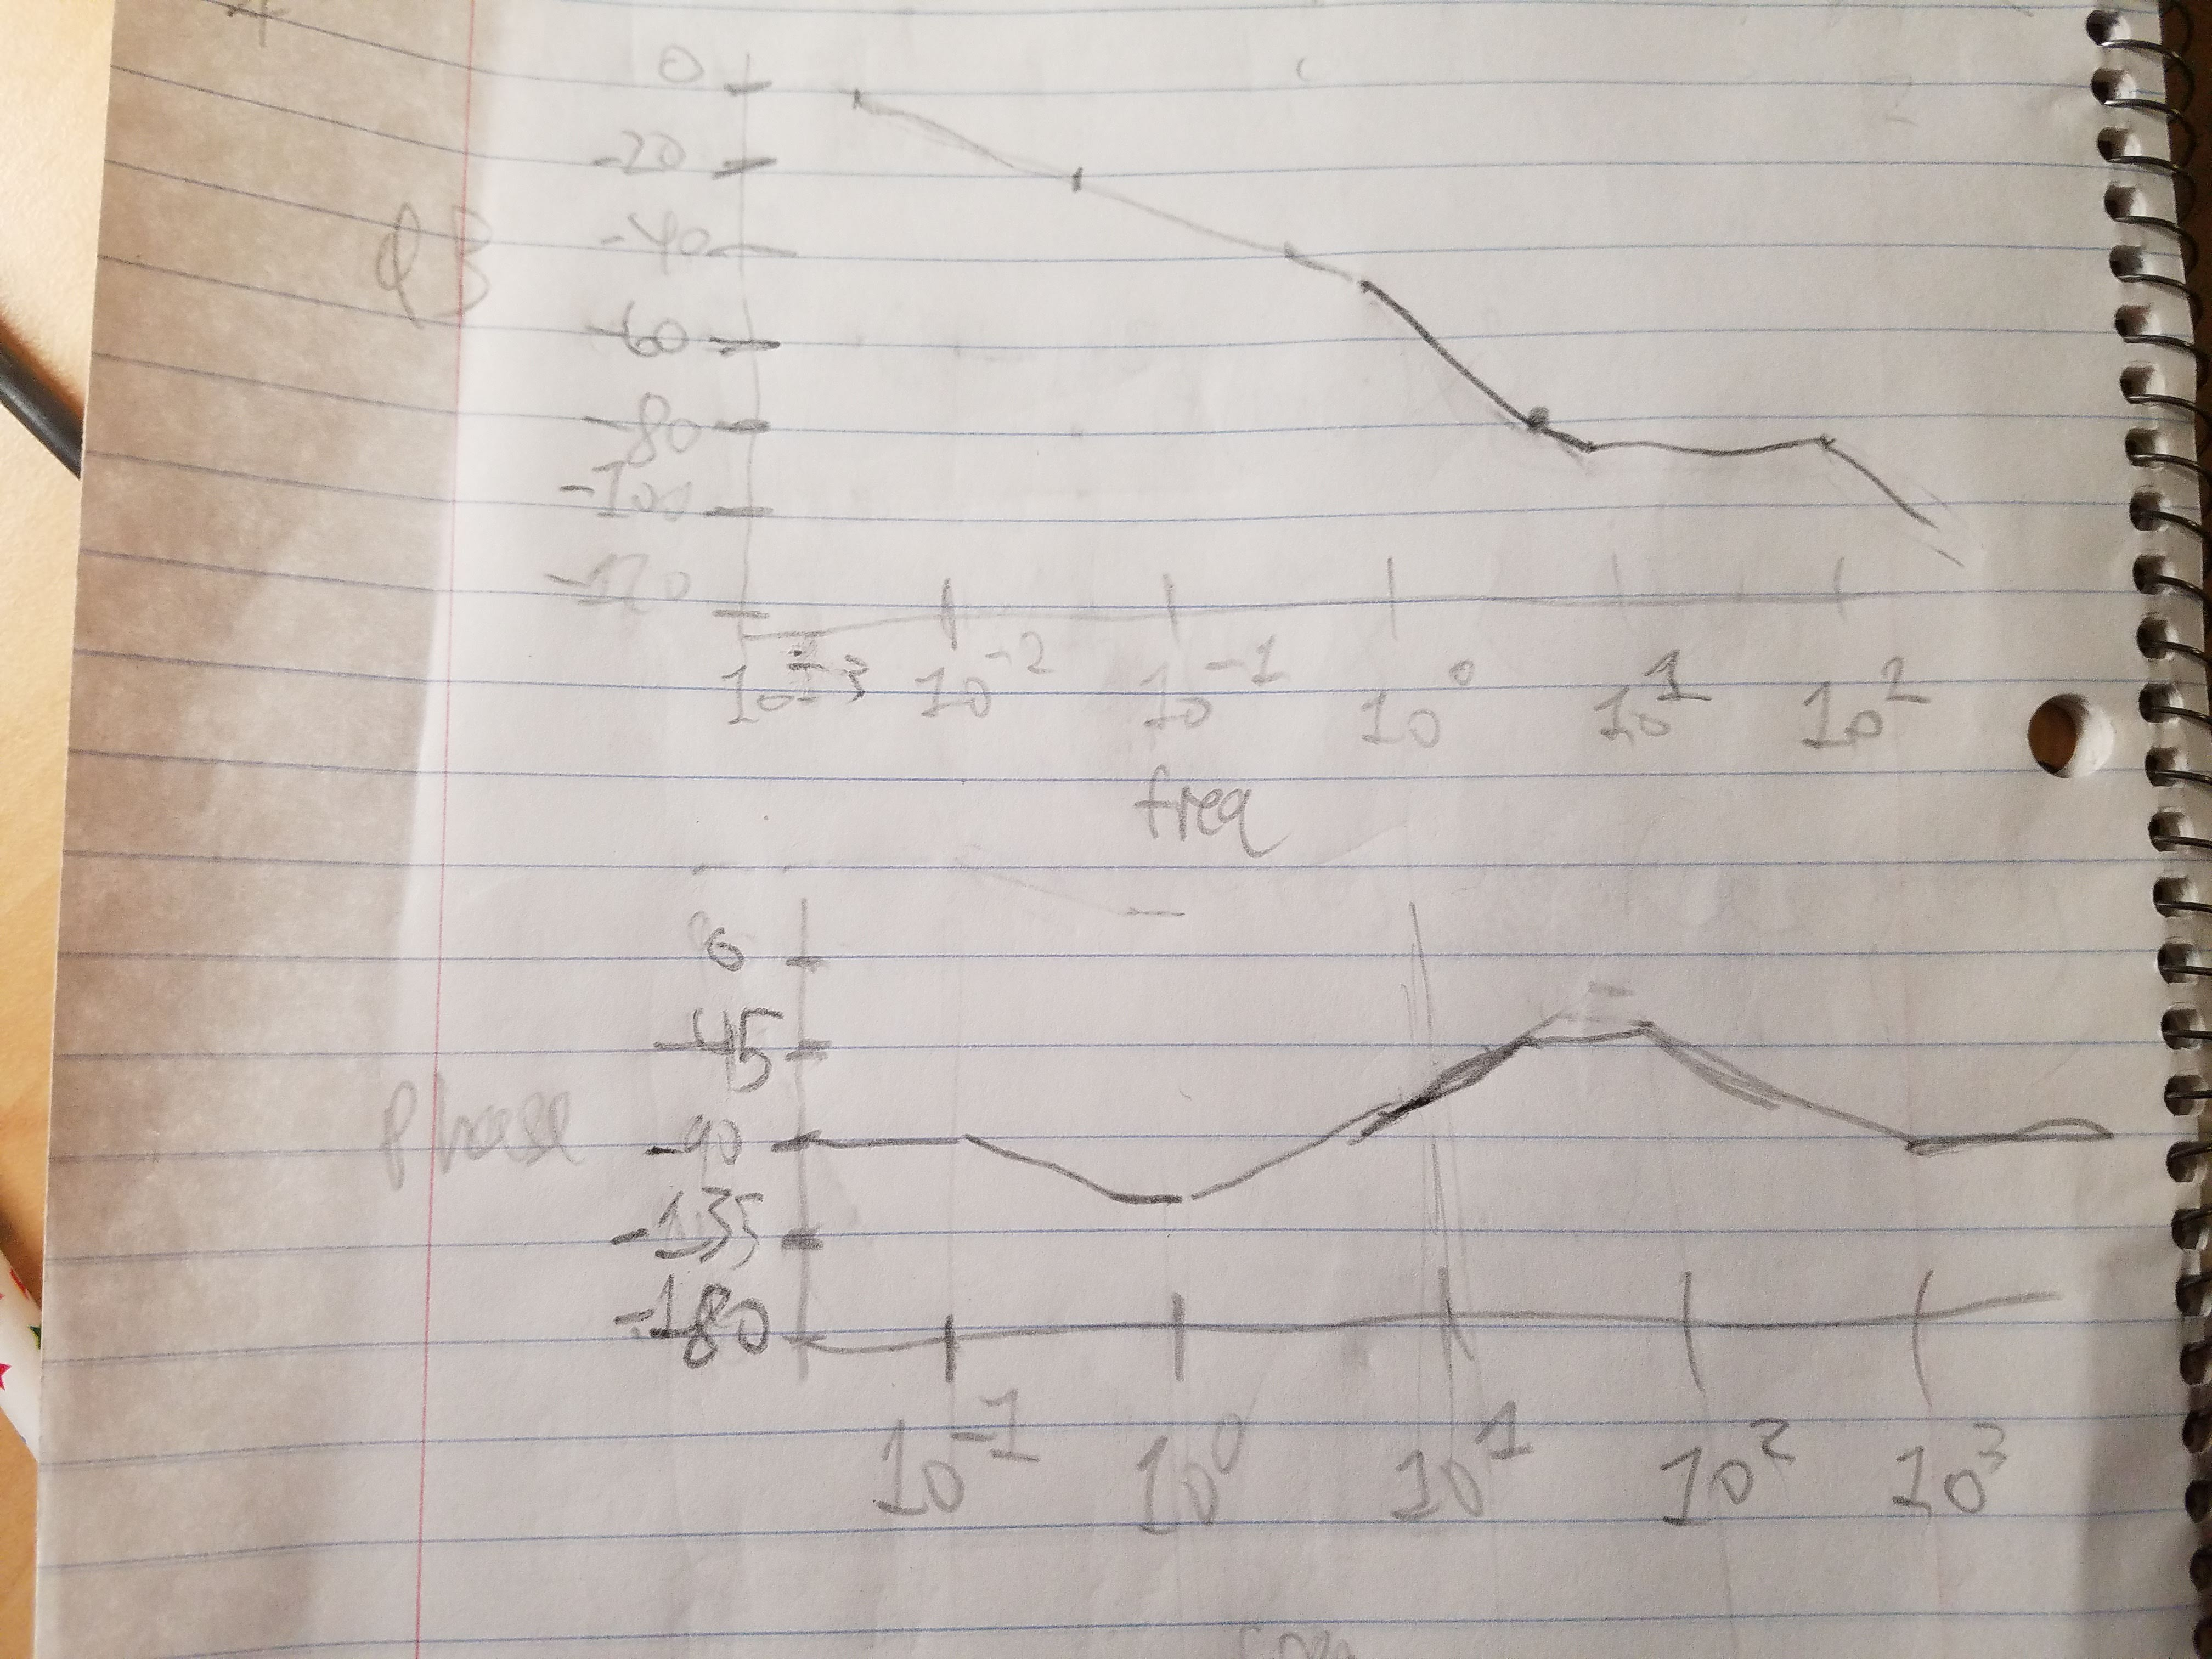
\includegraphics[width=3.5in]{problem1a.jpg}
    \end{center}
\end{figure}

\paragraph{b)}

This can be rewritten as follows.
\[L(s)=\frac{1}{s+1}\times\frac{1}{-s+1}\times s\]
The \(\frac{1}{-s+1}\) term produces the same magnitude as the first term but its phase goes to \(90\) instead of \(-90\) degrees since the imaginary component is reversed.
My asymptote sketch is shown below.
\begin{figure}[H]
    \begin{center}
        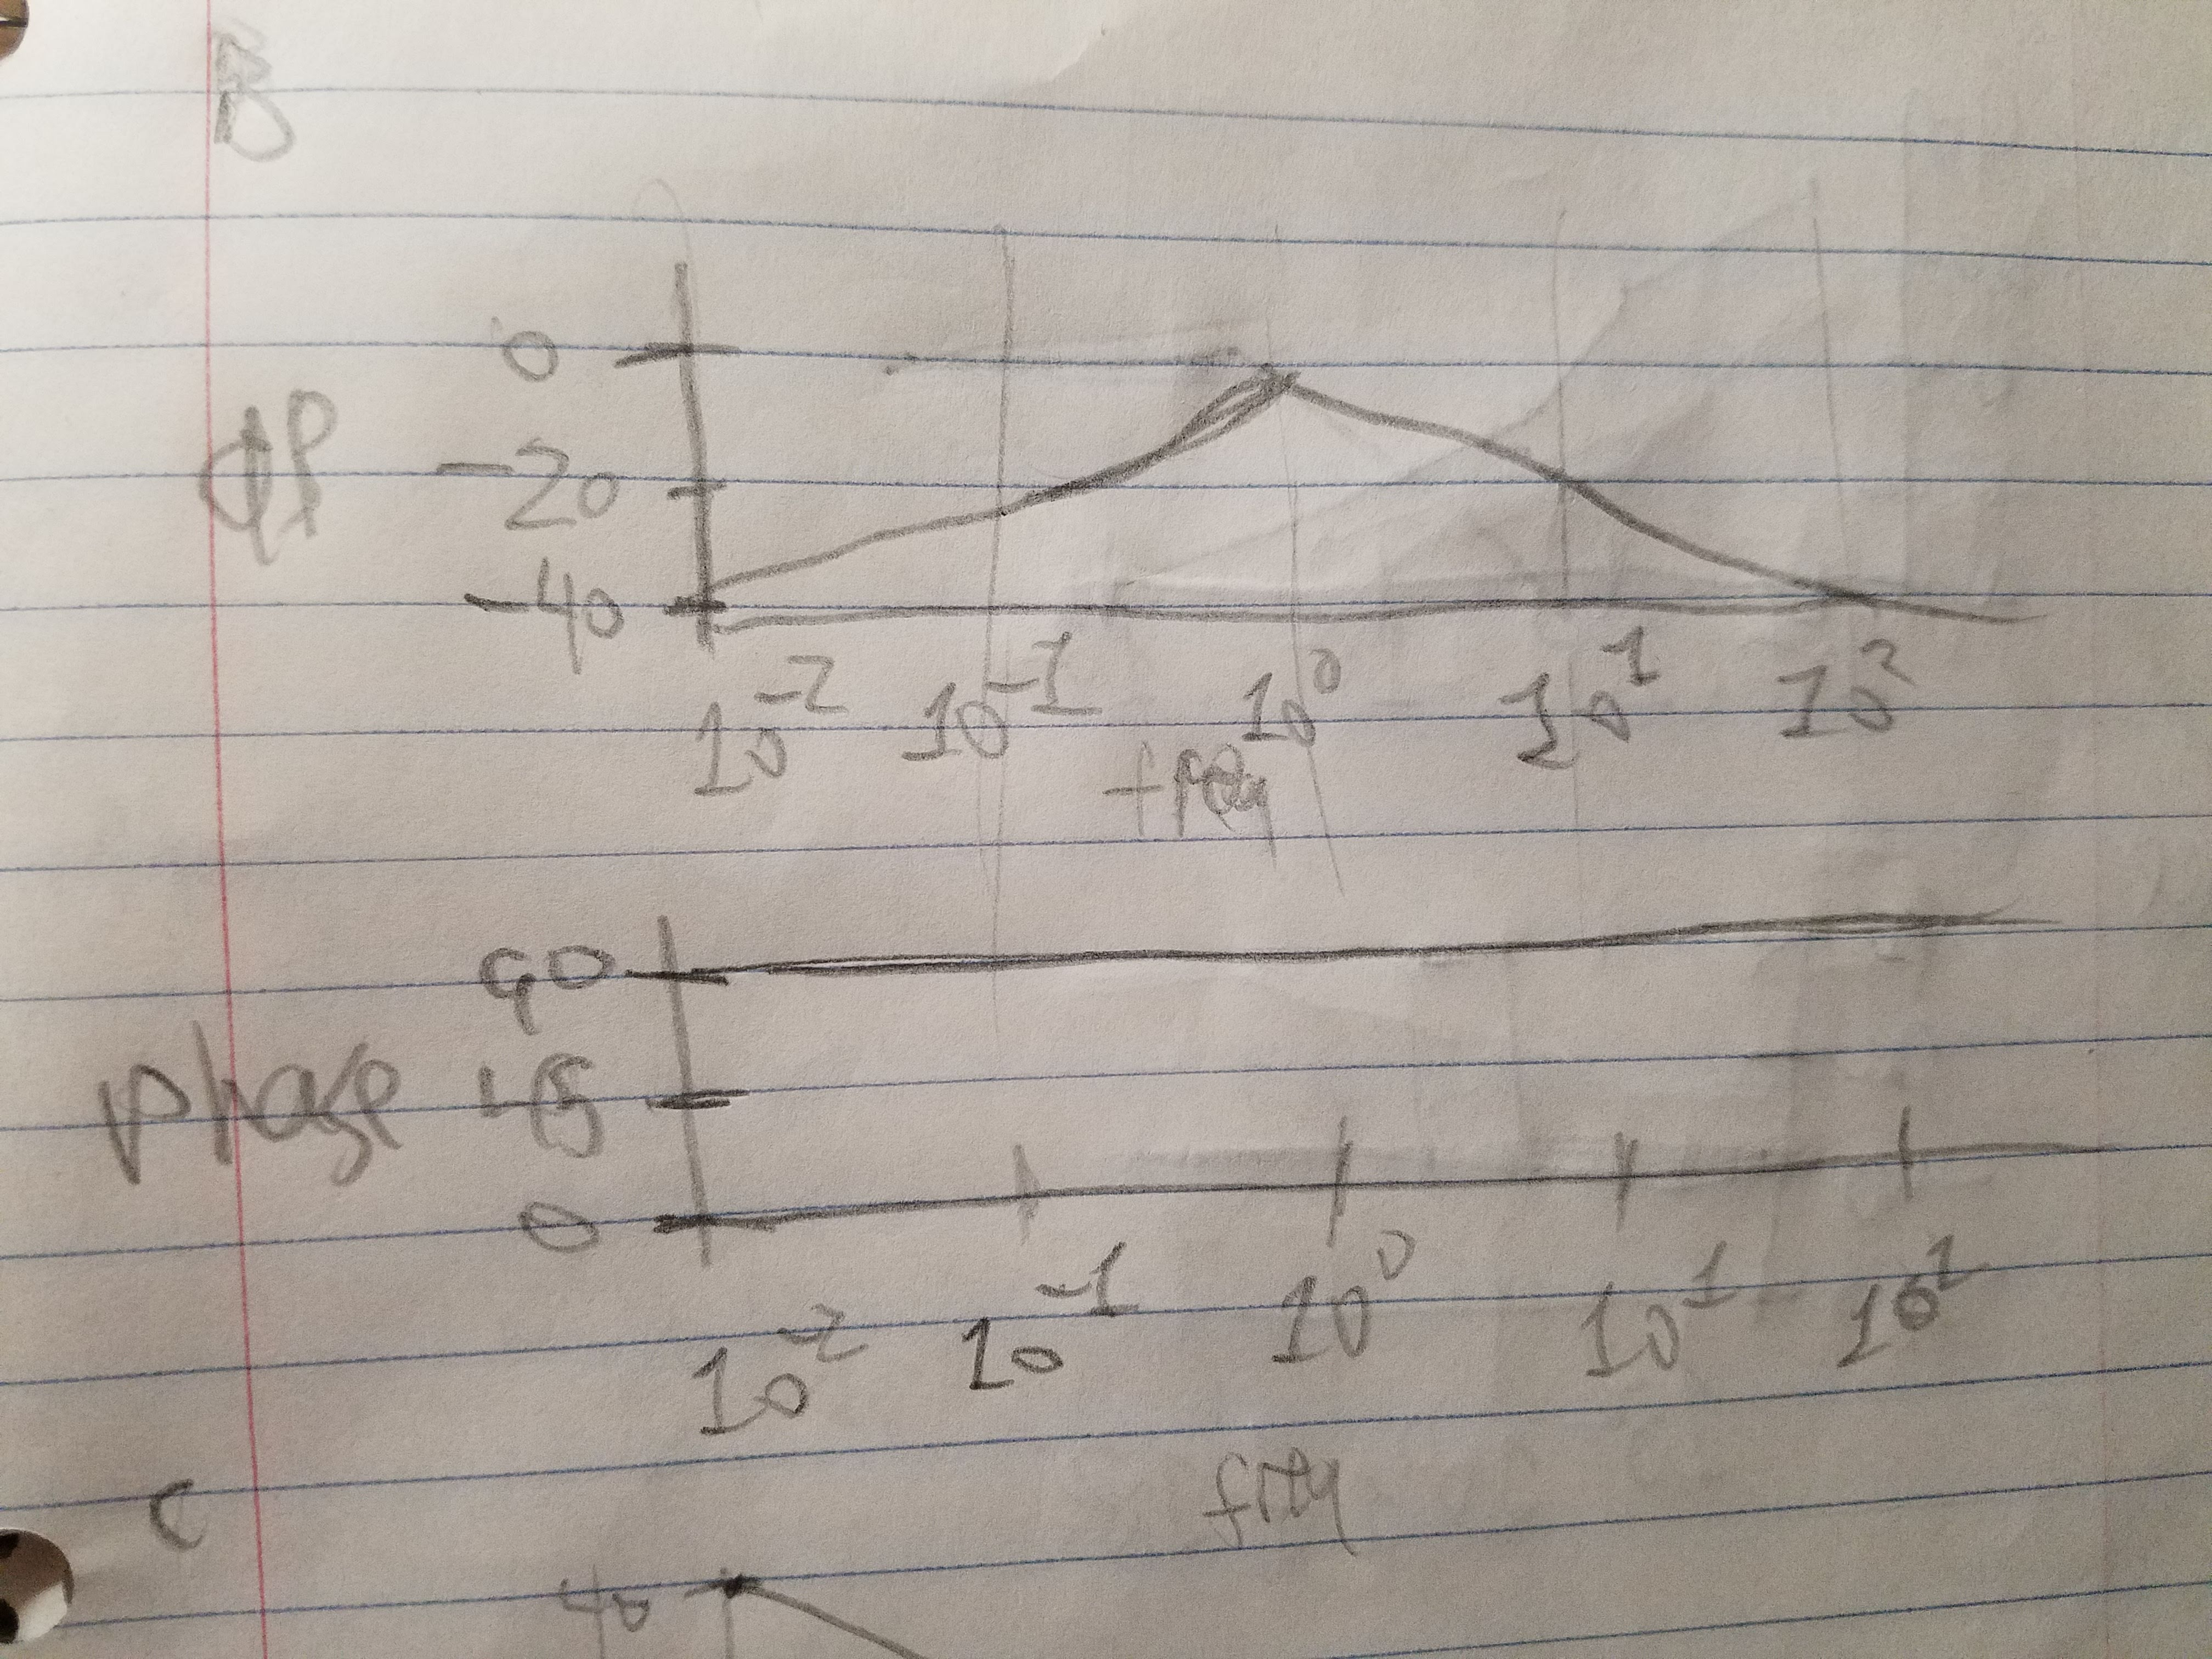
\includegraphics[width=3.5in]{problem1b.jpg}
    \end{center}
\end{figure}

\paragraph{c)}

This can be rewritten as follows.
\[L(s)=\frac{1}{s}\times\frac{1}{s+1}\times(-s+1)\]
The \(-s+1\) term has a phase that goes from 0 degrees to \(-90\) degrees since the imaginary component is reversed.
My asymptote sketch is shown below.
\begin{figure}[H]
    \begin{center}
        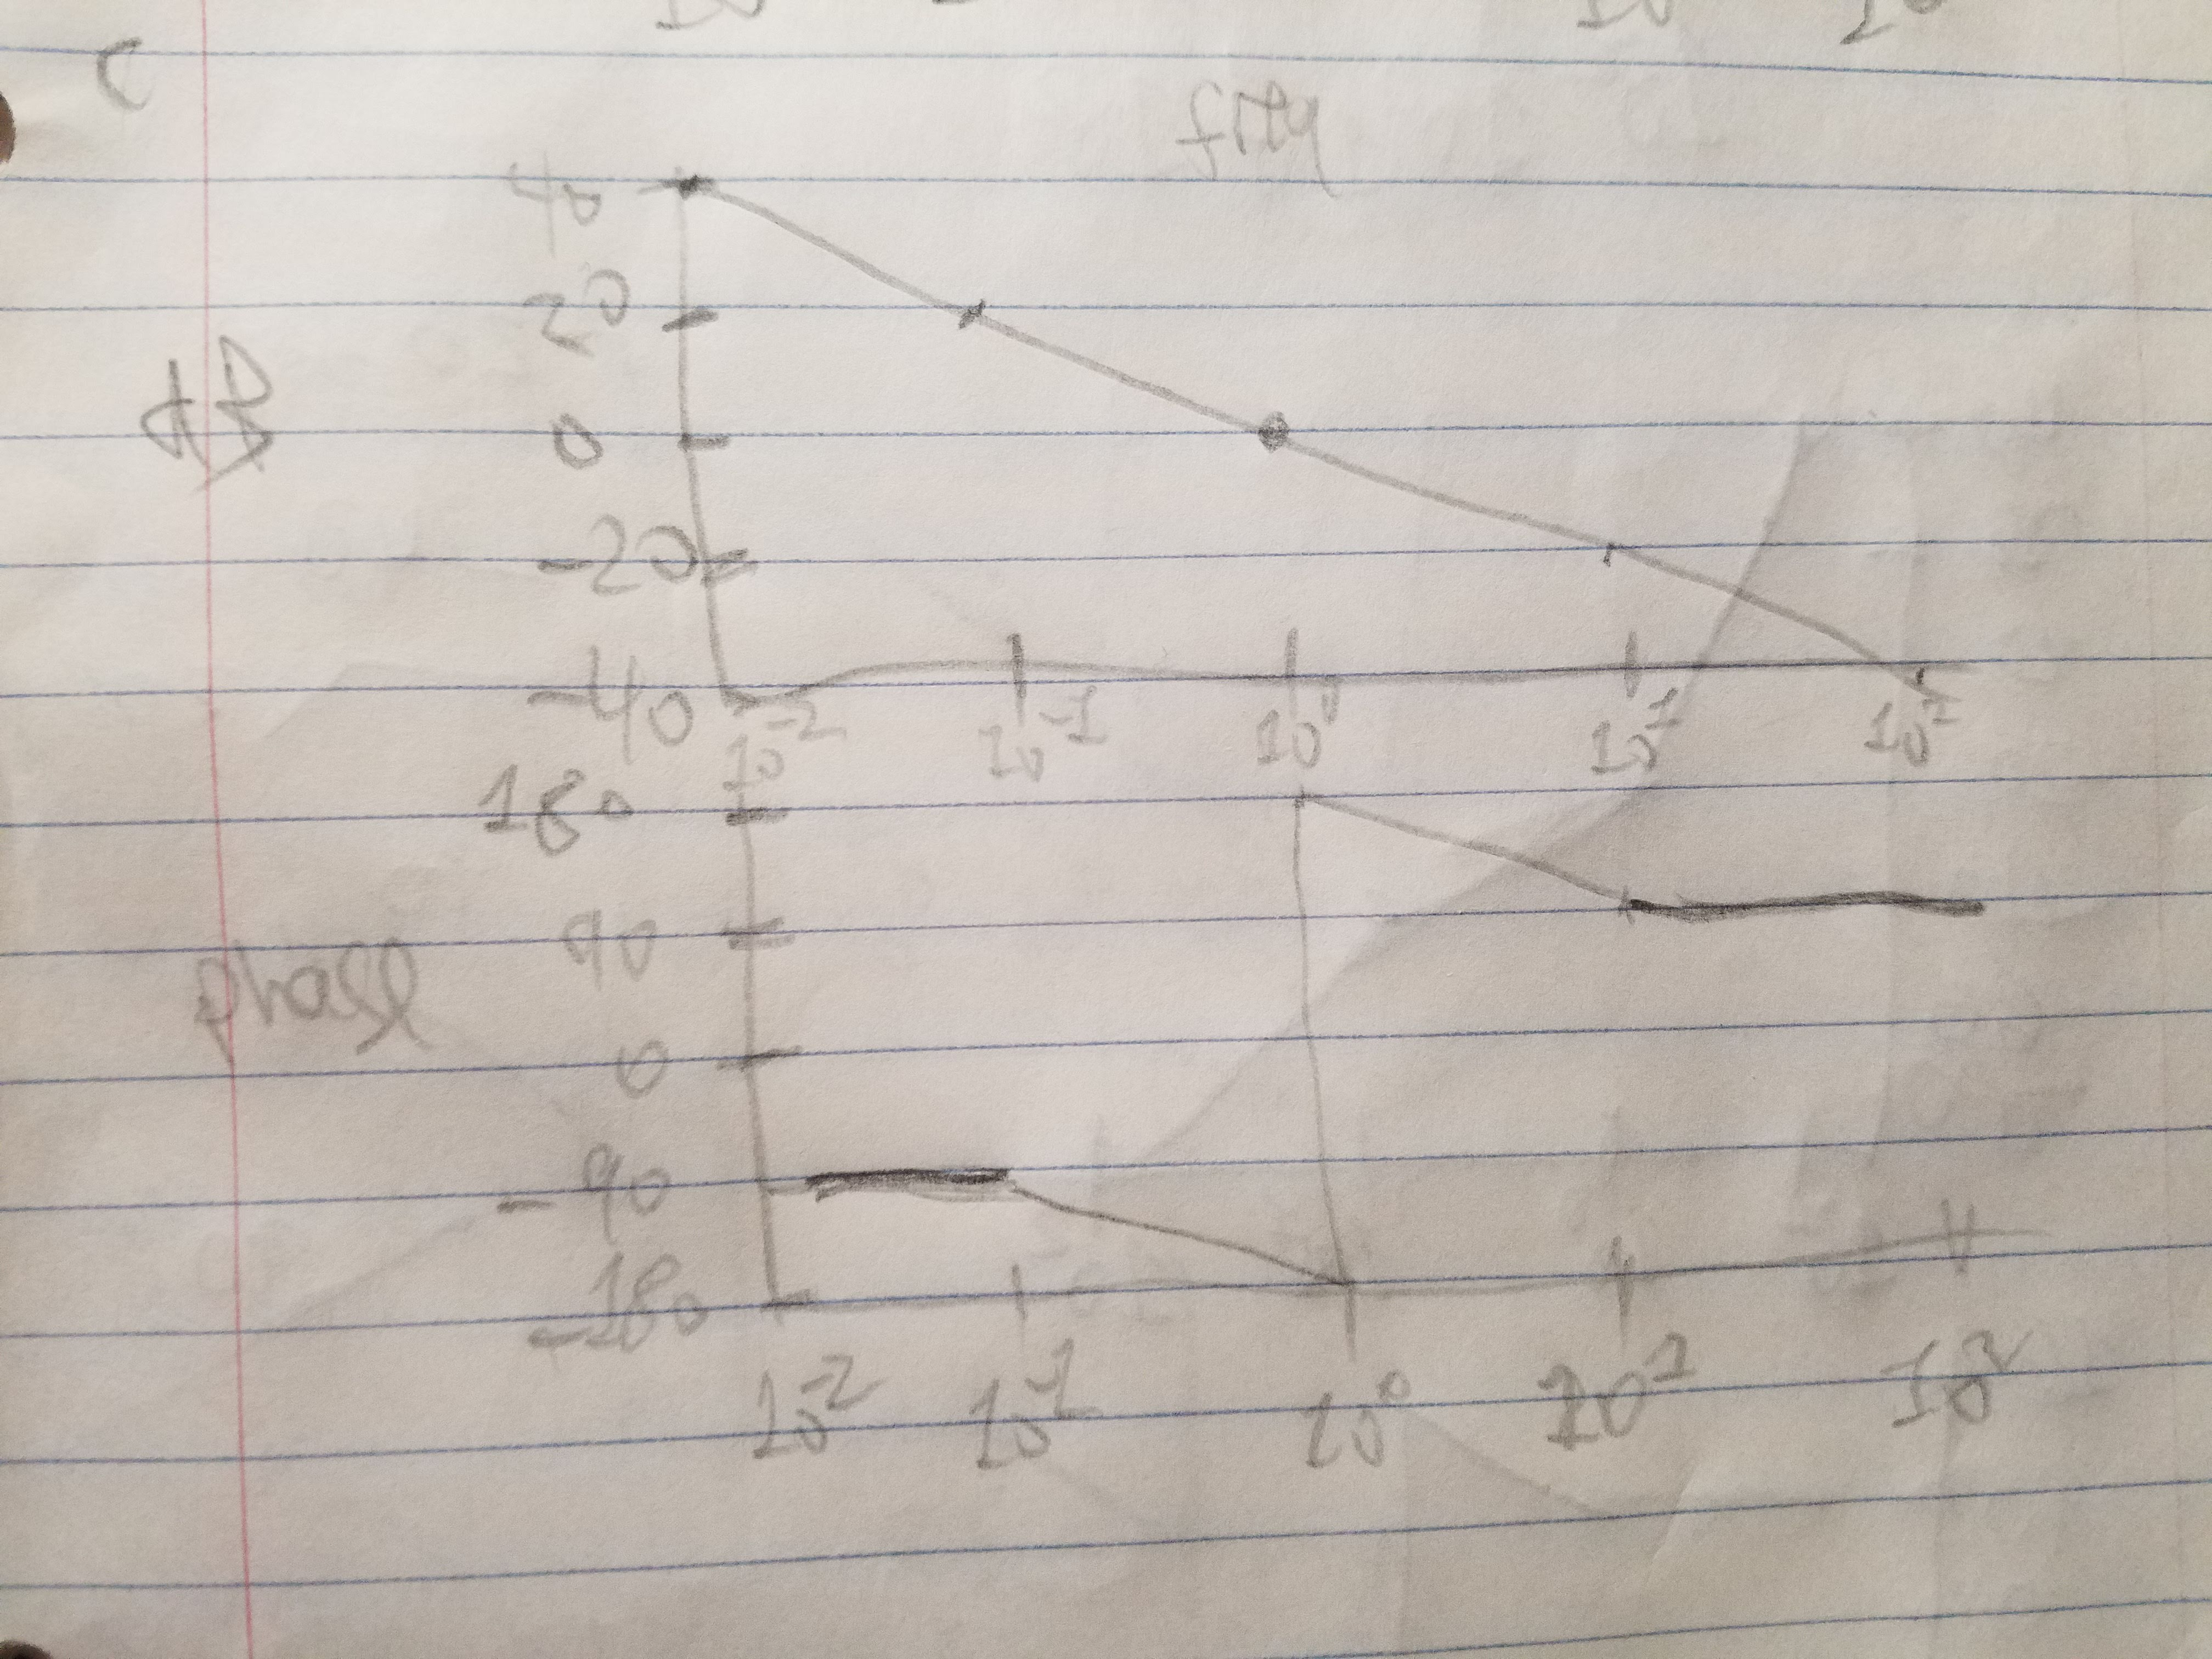
\includegraphics[width=3.5in]{problem1c.jpg}
    \end{center}
\end{figure}

\paragraph{d)}

This can be rewritten as follows.
\[L(s)=4\times\frac{1}{s}\times\frac{1}{s^2+1}\times\left(\left(\frac{s}{2}\right)^2+1\right)\]
The \(\frac{1}{s^2+1}\) term will have a phase that jumps immediately from 0 to \(-180\) after \(\omega=1\). Similarly
the quadratic term in the numerator will have a phase that jumps from 0 to \(180\) after \(\omega=2\). It has a magnitude asymptote
that increases at 40 decibels every decade after this point as well.
My asymptote sketch is shown below.
\begin{figure}[H]
    \begin{center}
        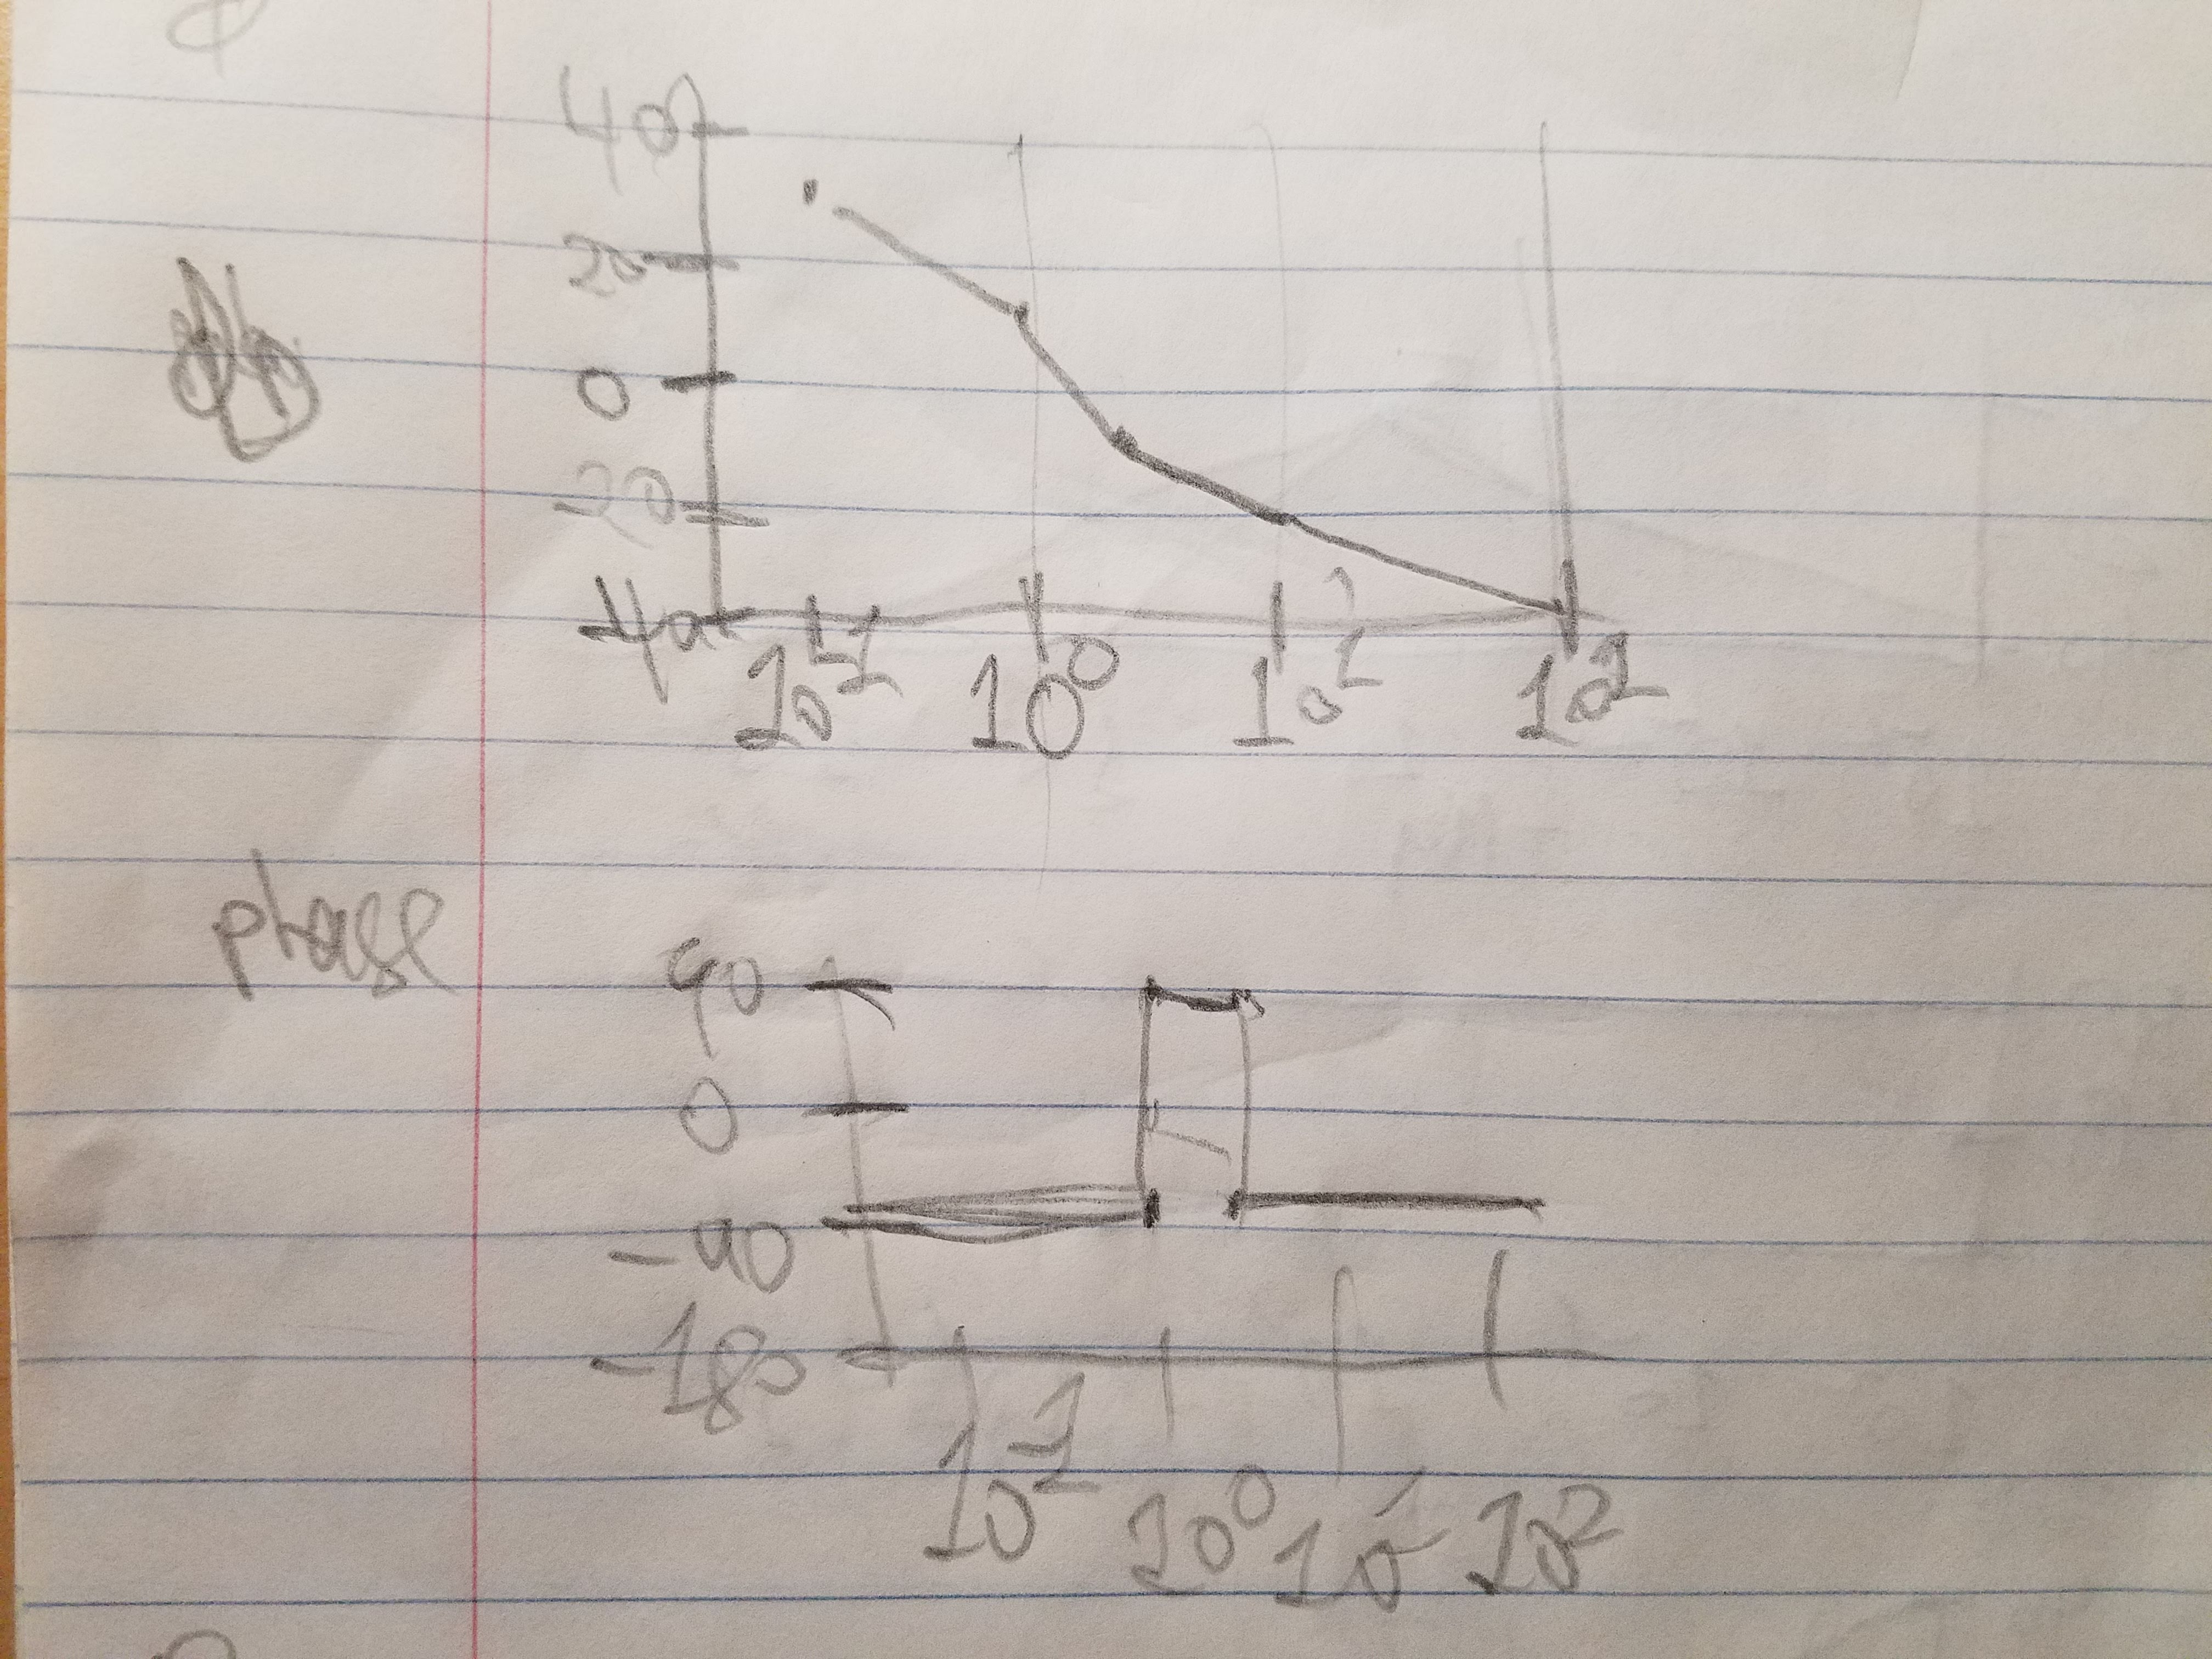
\includegraphics[width=3.5in]{problem1d.jpg}
    \end{center}
\end{figure}

\paragraph{e)}

This can be rewritten as follows.
\[L(s)=\frac{1}{10}\times\frac{1}{s^3}\times\frac{1}{\frac{1}{10}s+1}\times(s+1)\times(s+1)\]
My asymptote sketch is shown below.
\begin{figure}[H]
    \begin{center}
        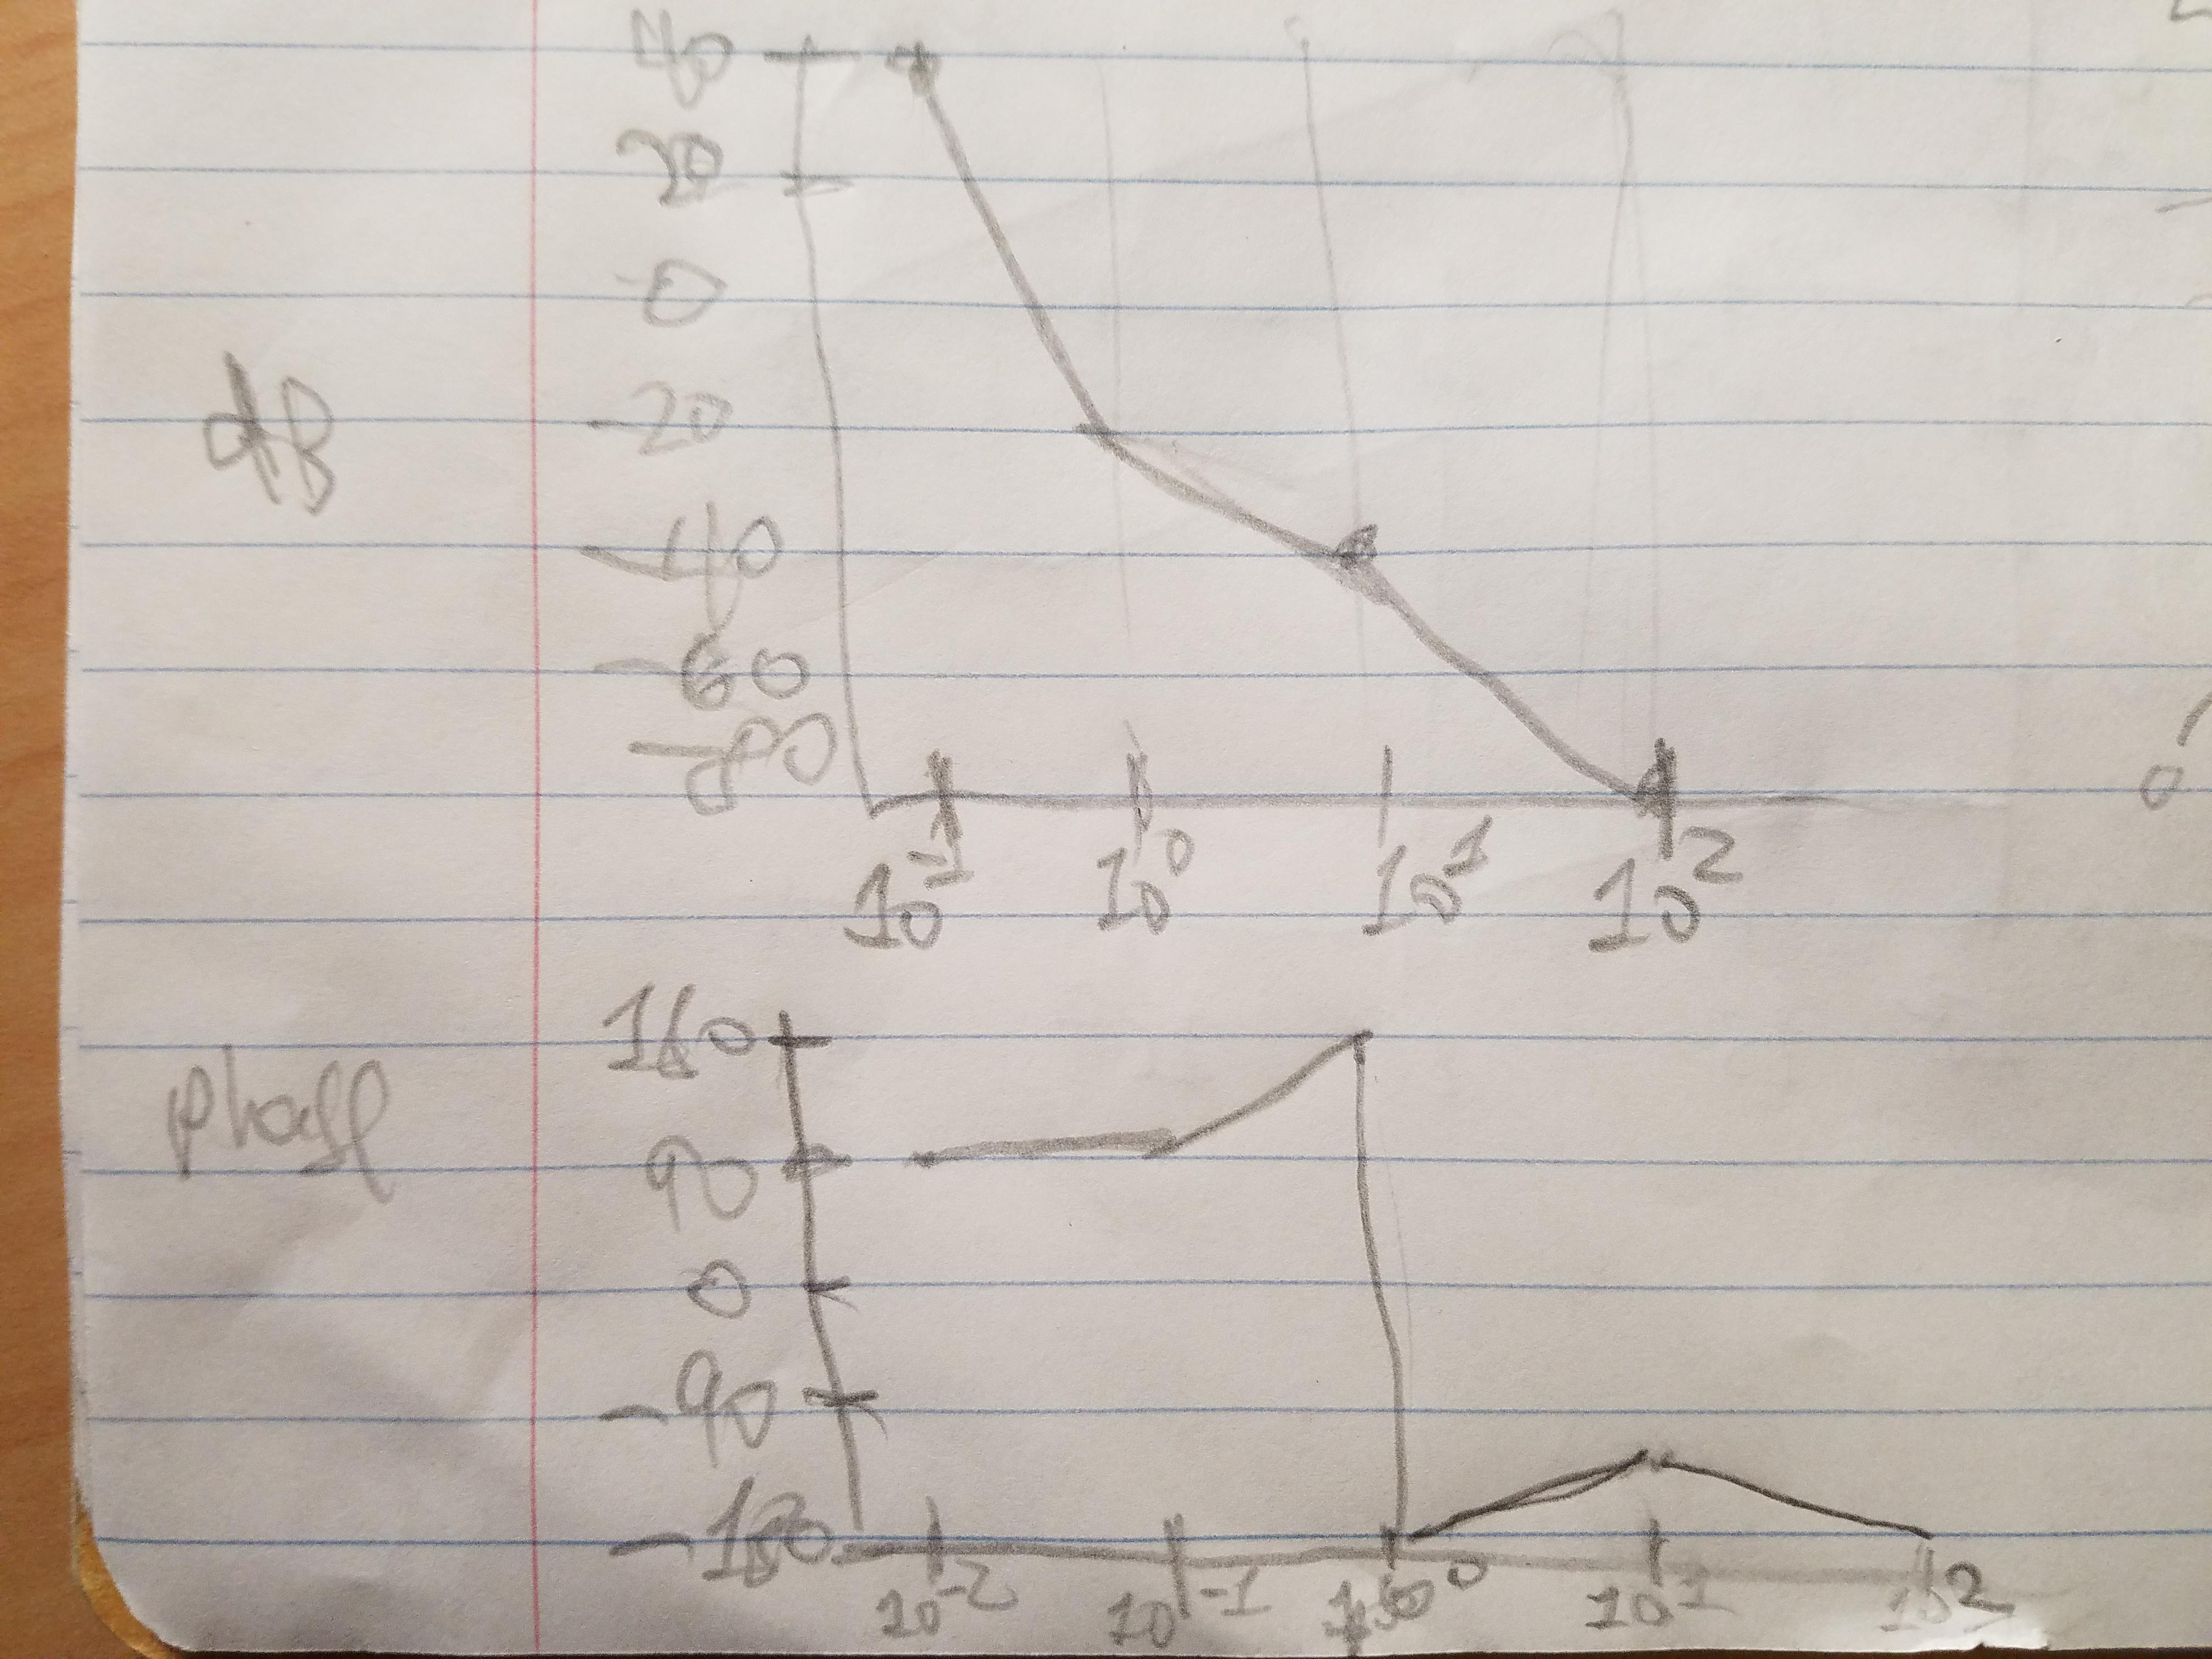
\includegraphics[width=3.5in]{problem1e.jpg}
    \end{center}
\end{figure}

\paragraph{f)}

This can be rewritten as follows.
\[L(s)=e^{-0.2s}\times\frac{1}{s}\times\frac{1}{s+1}\]
The exponential term has no effect on the magnitude. It will cause the phase to rapidly move cycle through all the angles as the frequency
increases, so there is no use predicting the asymptote for frequencies greater than 1.
My asymptote sketch is shown below.
\begin{figure}[H]
    \begin{center}
        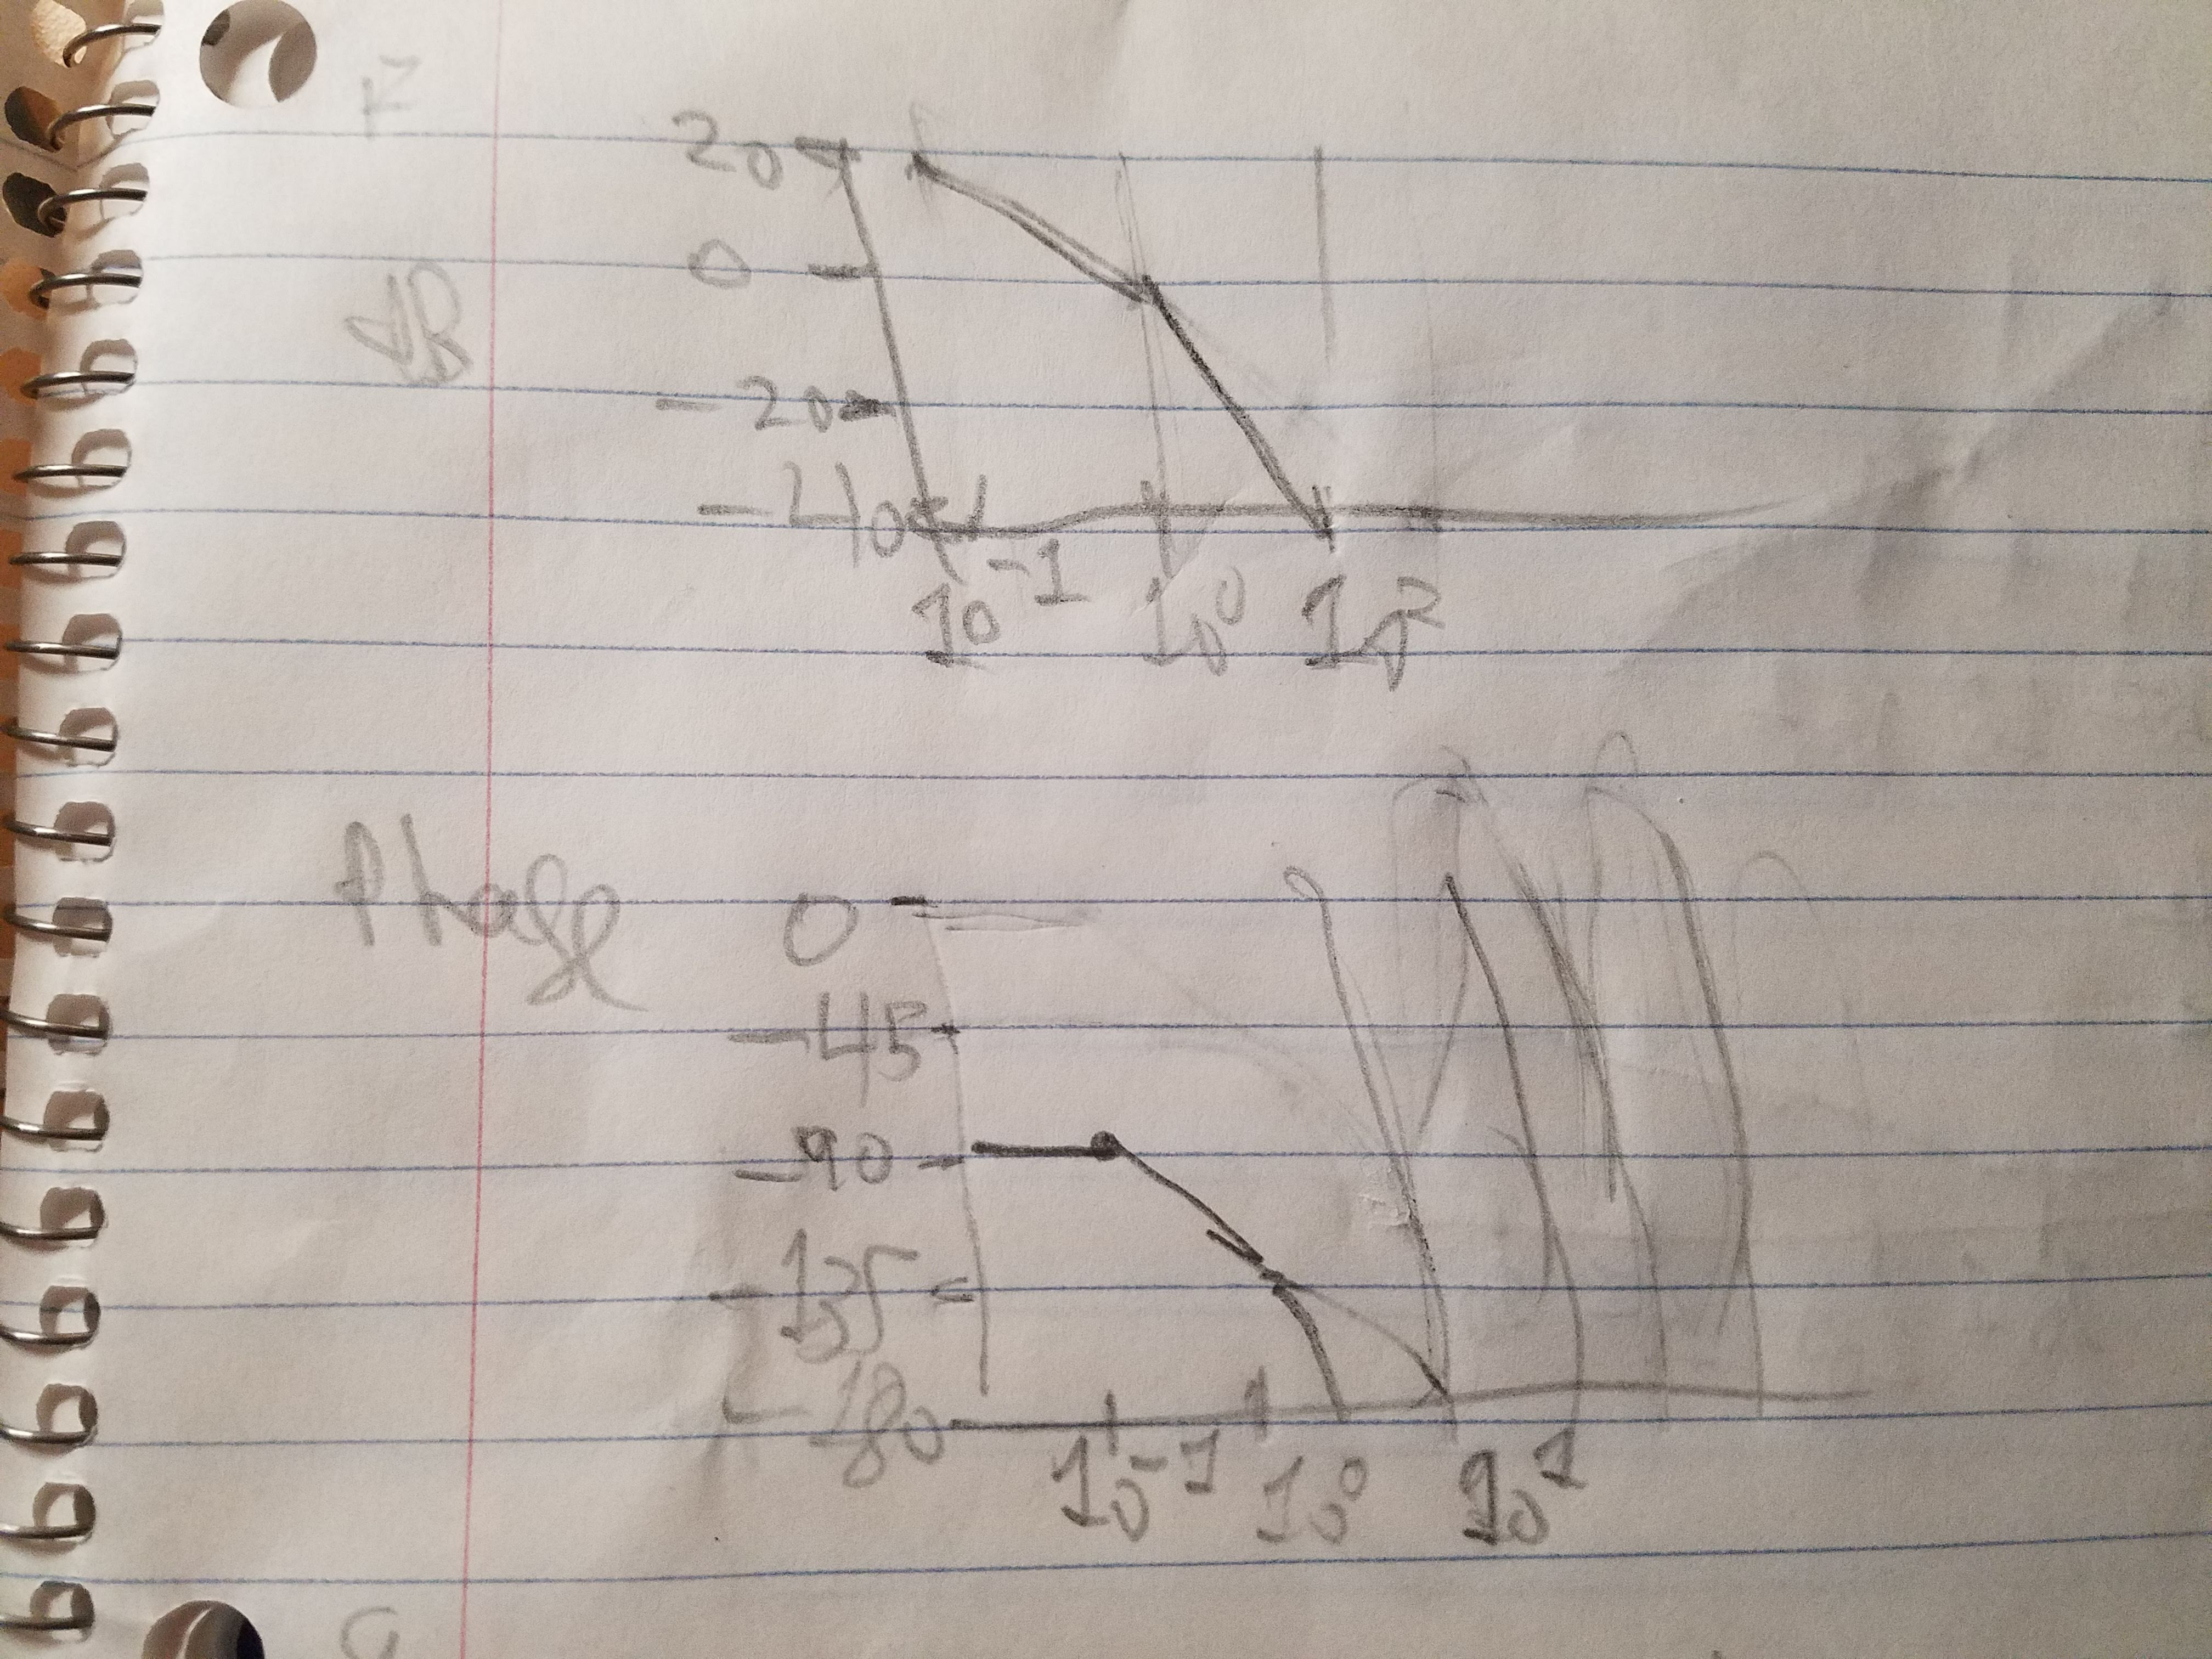
\includegraphics[width=3.5in]{problem1f.jpg}
    \end{center}
\end{figure}

\paragraph{g)}

This can be rewritten as follows.
\[L(s)=\frac{1}{10}\times\frac{1}{s}\times\frac{100}{s^2+20s+100}\times(s+1)\]
My asymptote sketch is shown below.
\begin{figure}[H]
    \begin{center}
        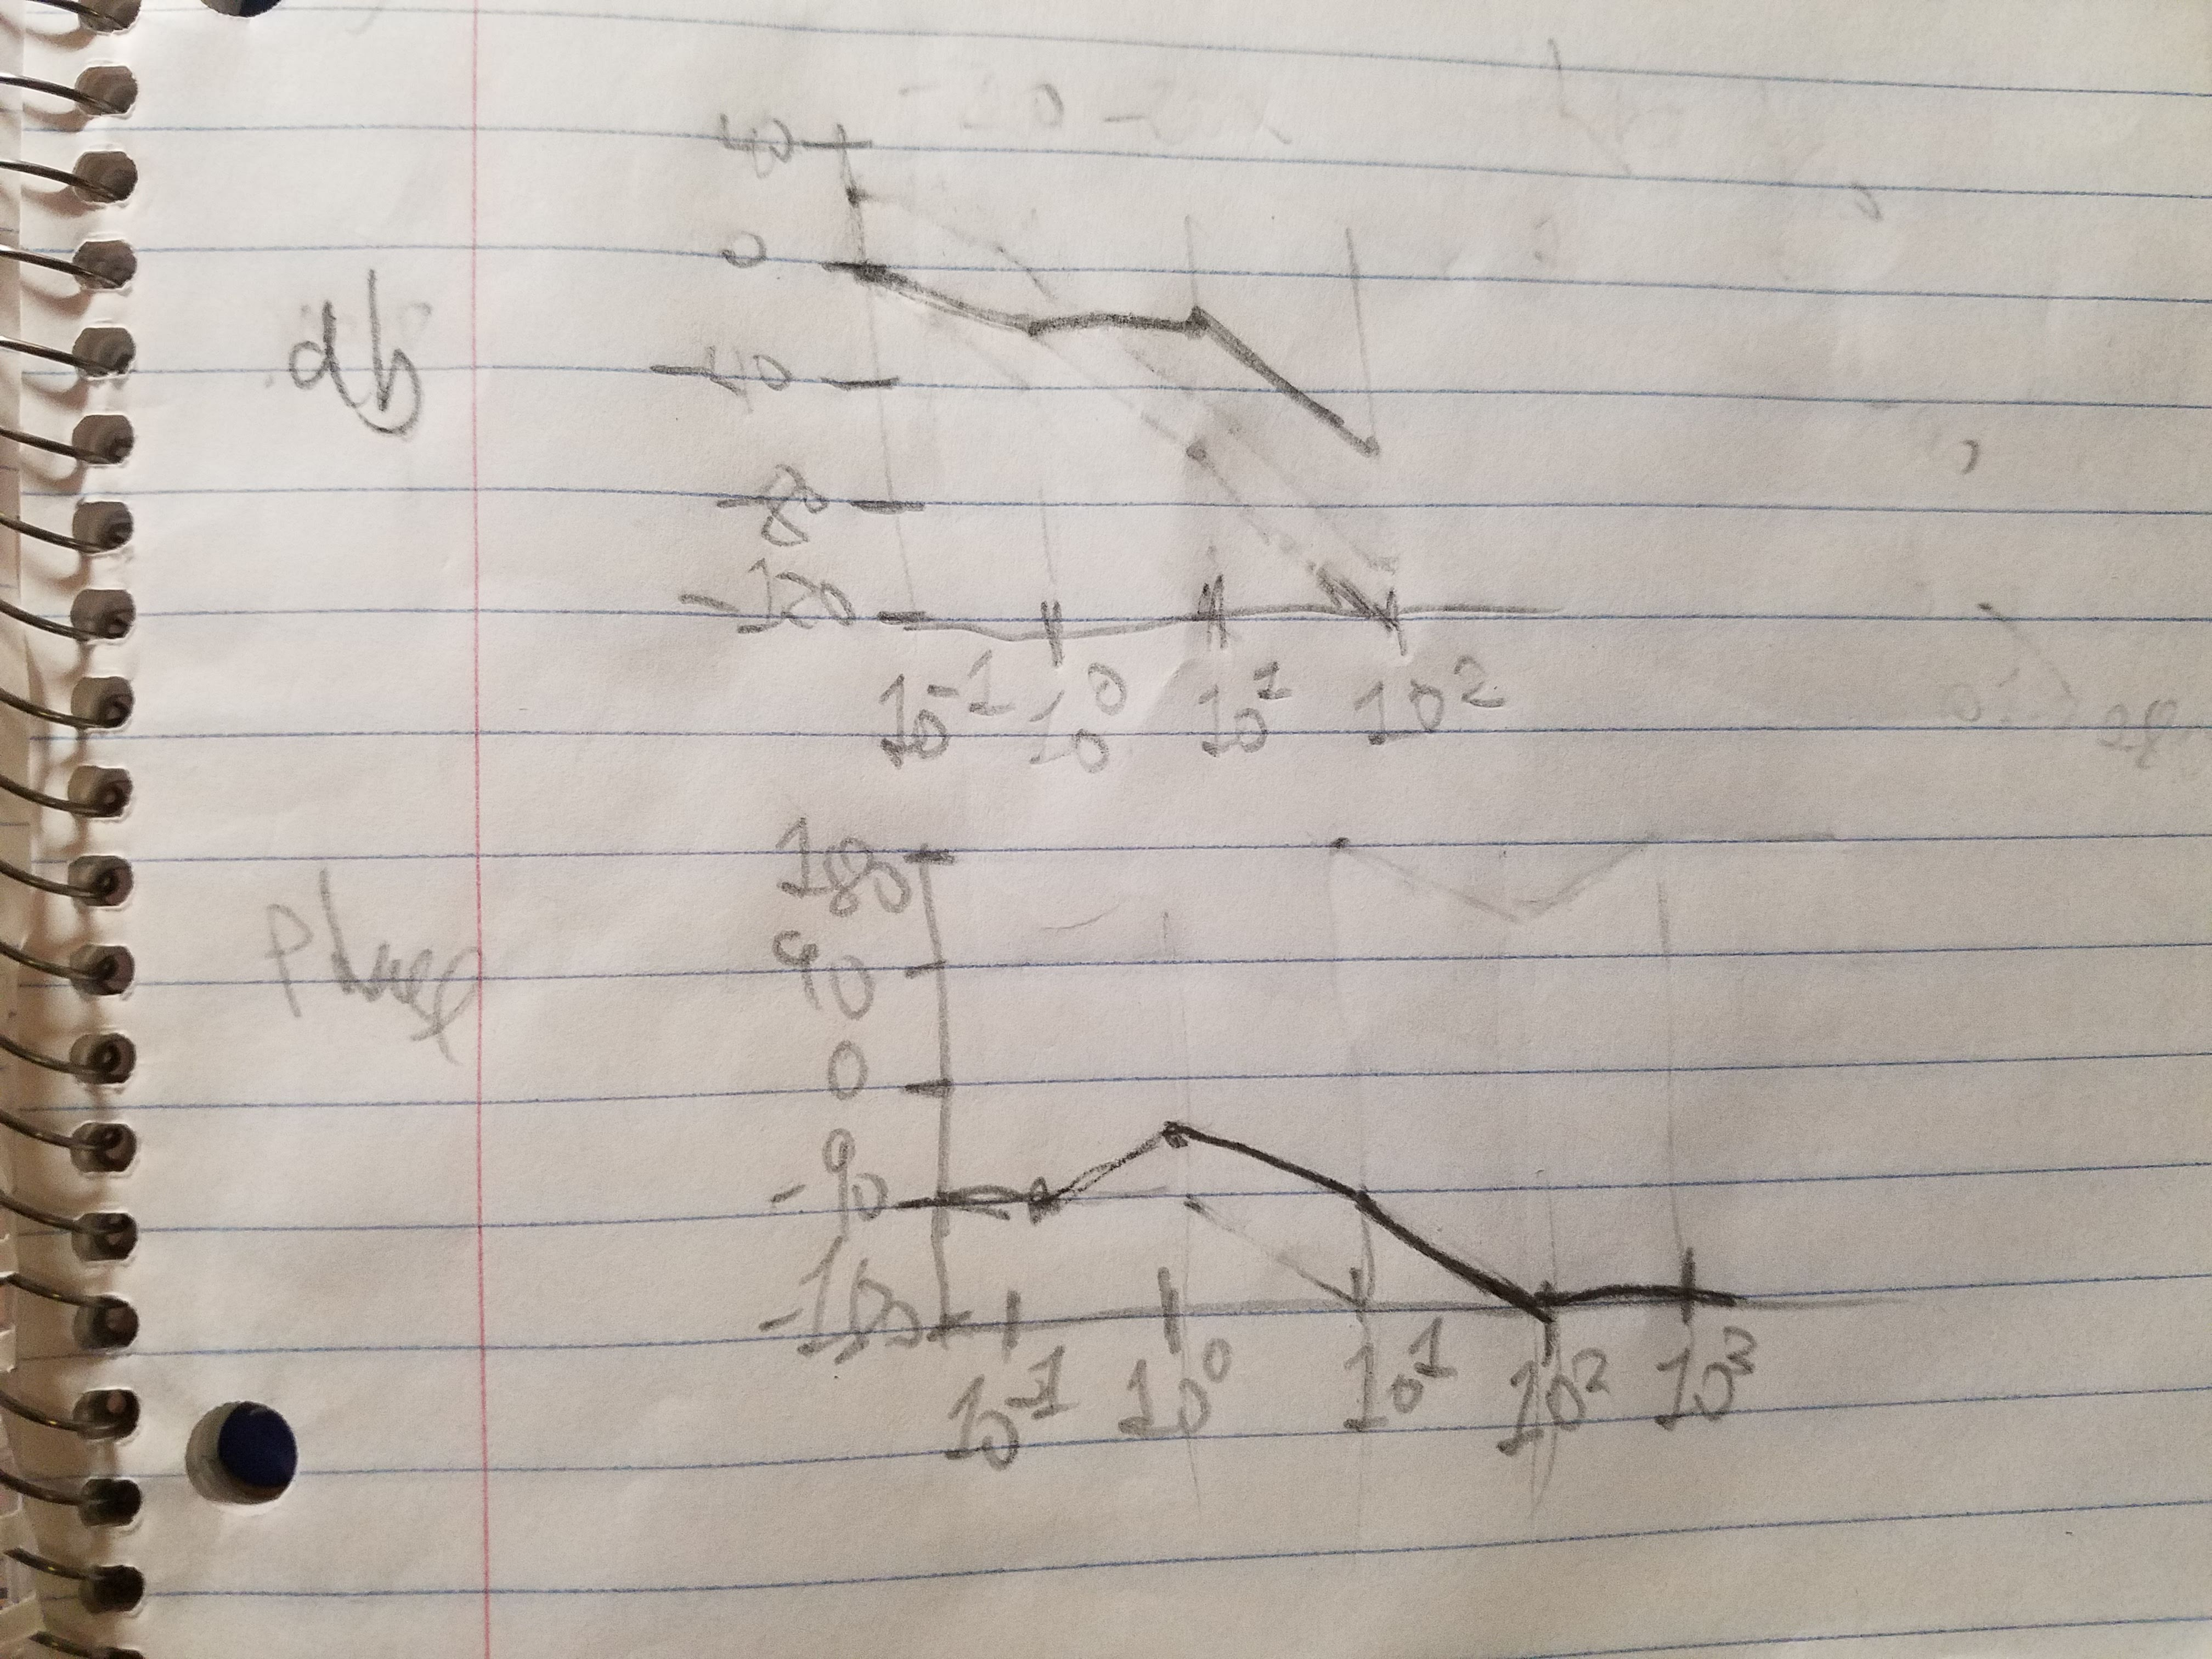
\includegraphics[width=3.5in]{problem1g.jpg}
    \end{center}
\end{figure}

\paragraph{h)}
This can be rewritten as follows.
\[L(s)=\frac{1}{s^2}\times\left(\frac{1}{2}s+1\right)\]
My asymptote sketch is shown below.
\begin{figure}[H]
    \begin{center}
        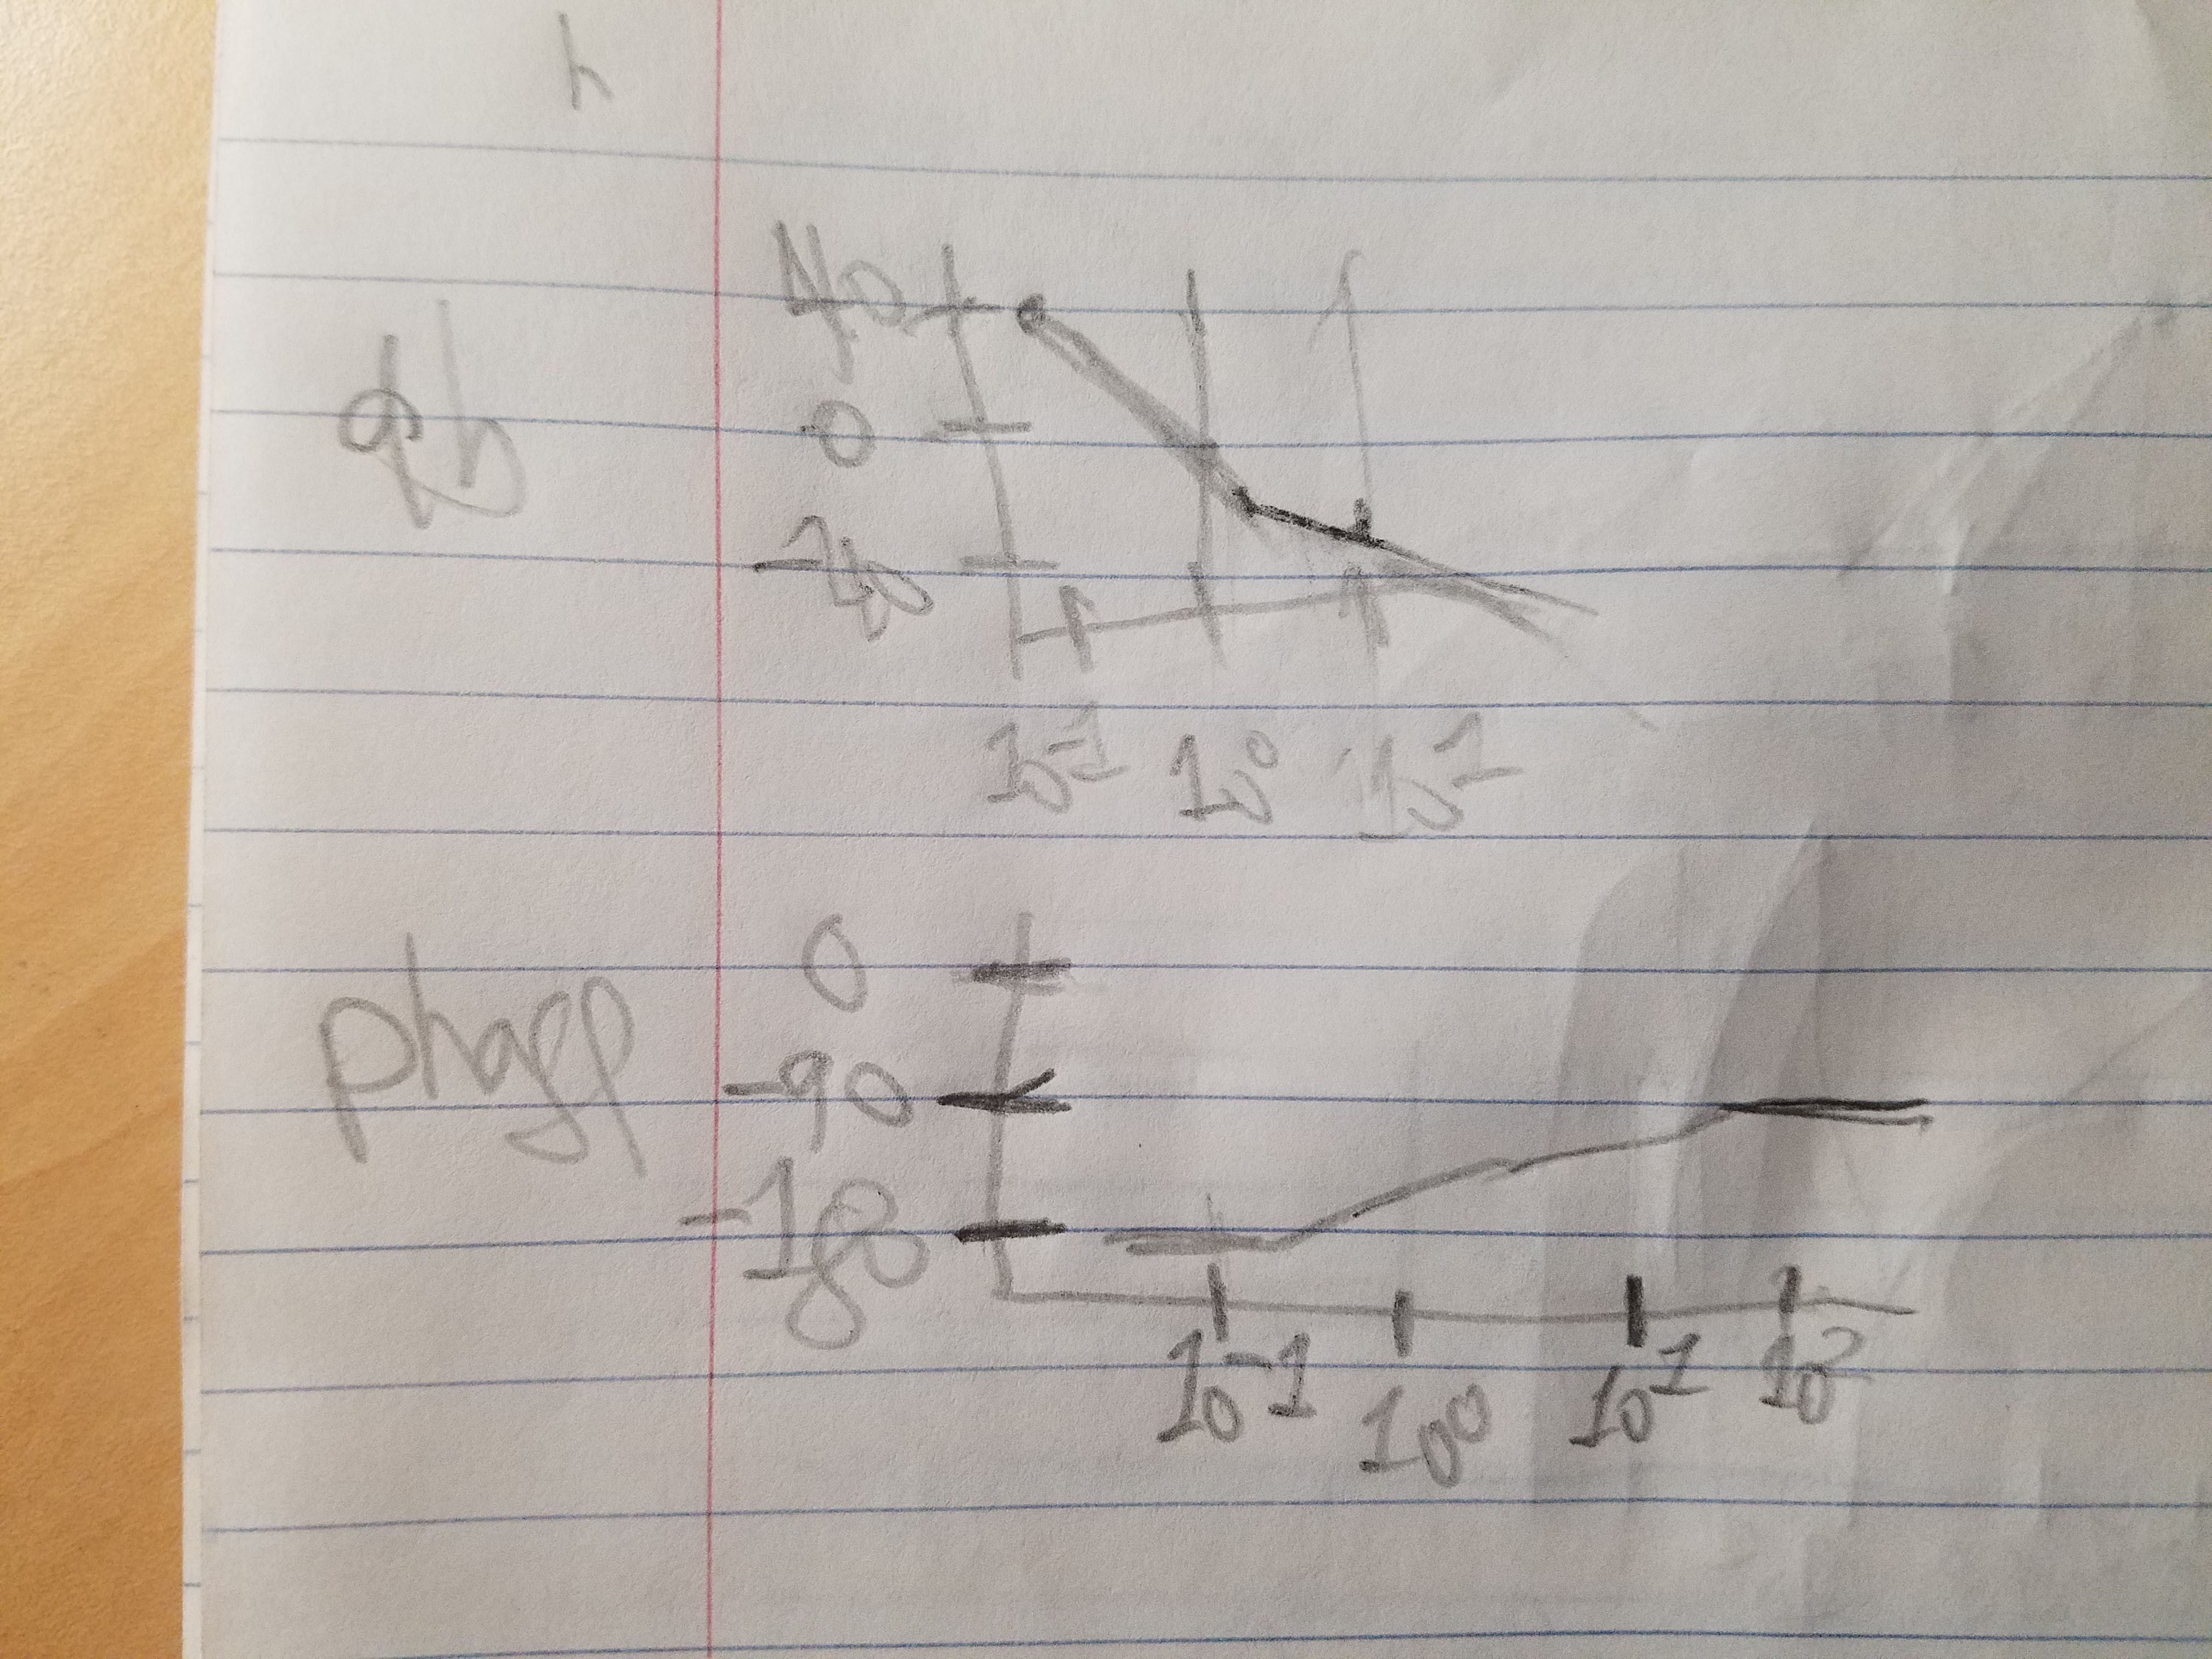
\includegraphics[width=3.5in]{problem1h.jpg}
    \end{center}
\end{figure}

\section*{Problem 2}

\paragraph{a)}

\paragraph{b)}

\paragraph{c)}

\paragraph{d)}

\paragraph{e)}

\section*{Problem 3}

\paragraph{a)}

\paragraph{b)}

\paragraph{c)}

\paragraph{d)}

\paragraph{e)}

\section*{Problem 4}

\paragraph{a)}

\paragraph{b)}

\paragraph{c)}

\paragraph{d)}

\section*{Problem 5}

\paragraph{a)}

\paragraph{b)}

\paragraph{c)}

\section*{Problem 6}

\paragraph{a)}

\paragraph{b)}

\paragraph{c)}

\end{document}